\documentclass{article}
\usepackage[utf8]{inputenc}
\usepackage{amsmath}
\usepackage{siunitx} 
\usepackage{pdfpages}
\usepackage[citestyle=numeric,bibstyle=authortitle]{biblatex}
\addbibresource{./lit.bib}
\usepackage{amsmath}
\usepackage[main=ngerman, english]{babel}
\usepackage{graphicx} % for image support
\usepackage{geometry} % Für schmale Seitenränder
\usepackage{physics} % $\bra{\Psi}\ket{\Psi}$ $\expval{A}{\Psi}$
\usepackage{braket} % $\braket{0|0}$    (Überschreibt die \braket Funktion des physics-Pakets!) 
\usepackage{caption}
\usepackage{subcaption}
 \geometry{
 a4paper,
 total={170mm,257mm},
 left=20mm,
 top=20mm,
 }

\graphicspath{ {./Images/} }

% Commands
\newcommand{\dee}{\mathop{\mathrm{d}\!}}


%\title{F1-Vorlage}
%\author{Autor 1, Autor 2}
%\date{October 2022}


\begin{document}
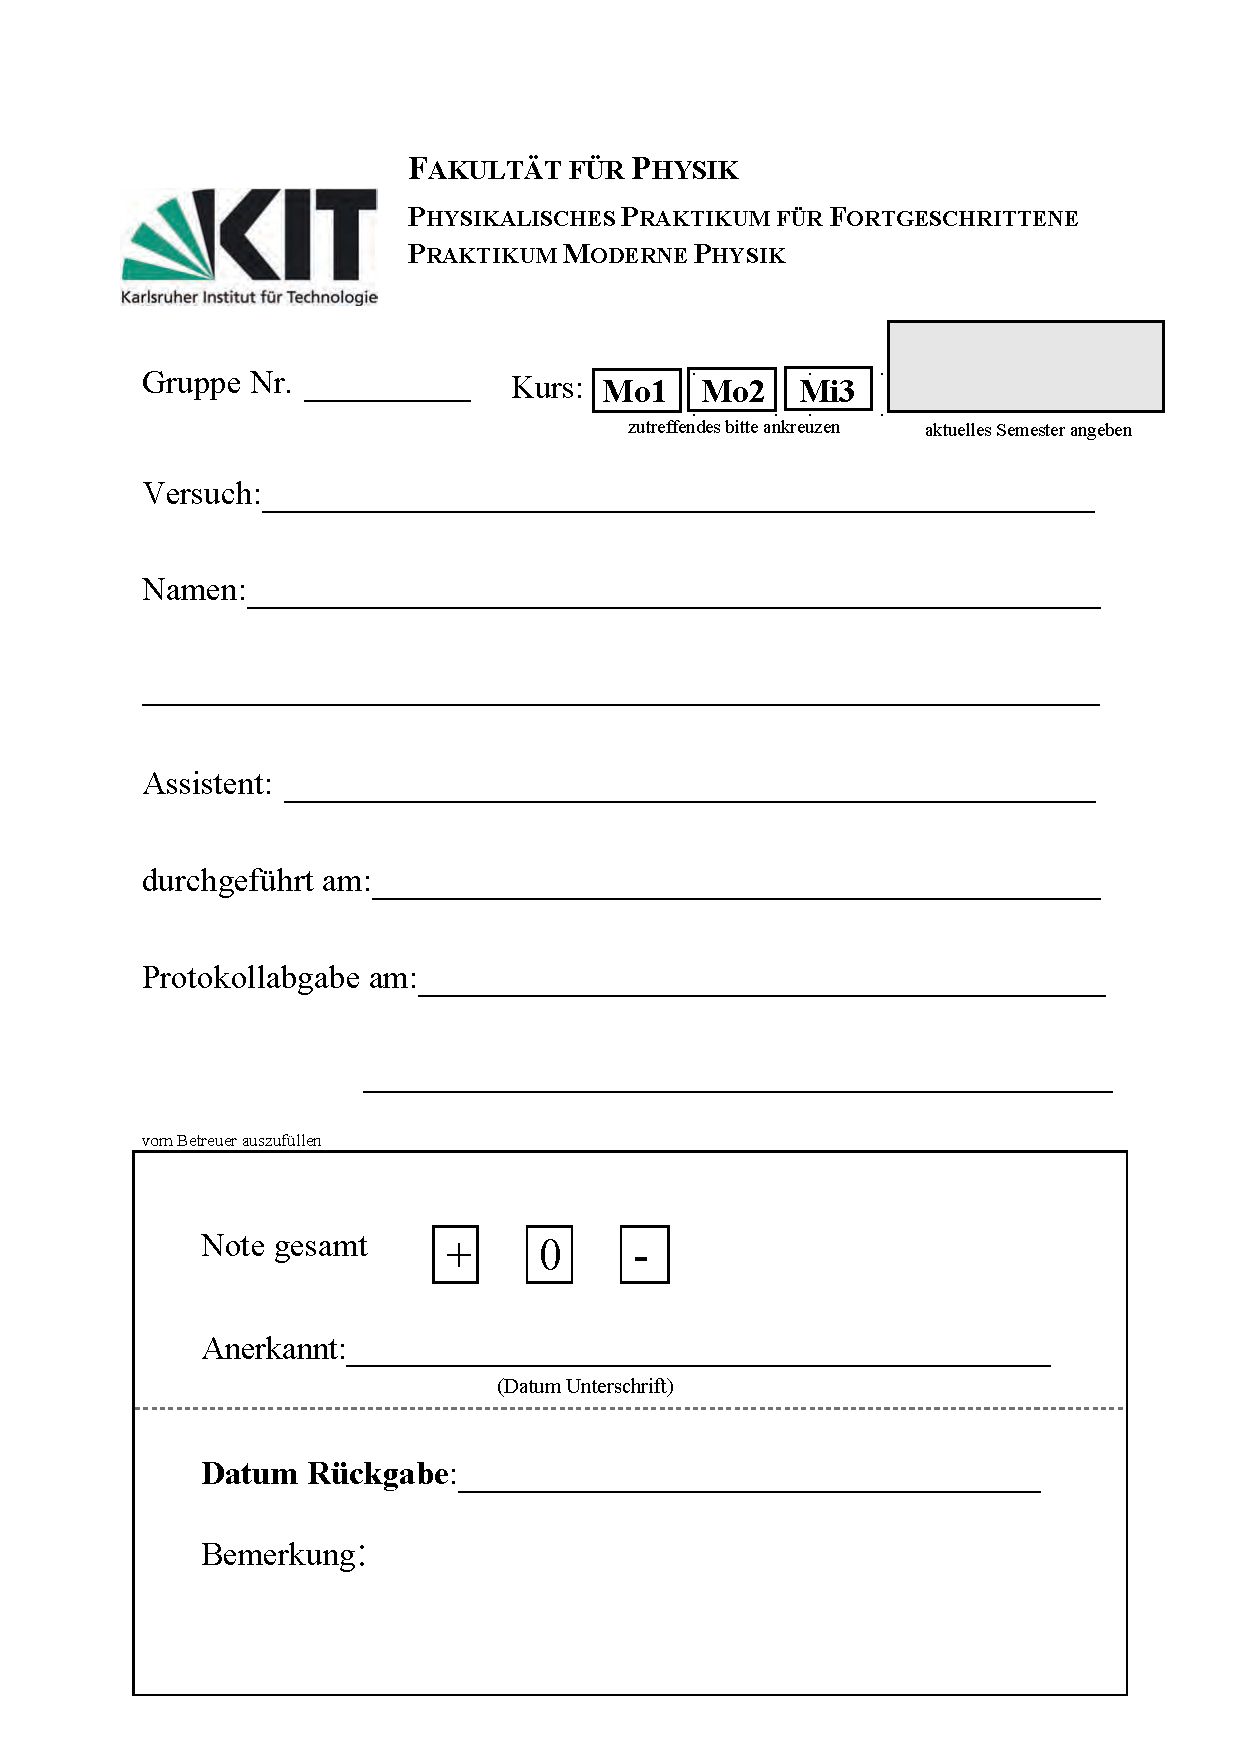
\includepdf[pages=1, offset=0 0]{./Deckblatt/raster.pdf} % Das pdf "Deckblatt/zum ausfuellen.pdf" muss gerastert exportiert werden damit Kommentare sichtbar weren

% INHALTSVERZEICHNIS
\setcounter{page}{1}
%\maketitle
\tableofcontents
\newpage

\section{/Erstes Kapitel}
%Beispiel \cite{Dem10}


\begin{gather*}
    \braket{A|B} \\
    \bra{\Psi}\ket{\Psi}\\
    \expval{A}{\Psi}
\end{gather*}


\newpage
%\printbibliography
\end{document}
